\subsection{Kinematic Region Definition}
\label{sec:selection:region}

The final cut defining our signal region uses \Xhh as given by \Eqn{\ref{eq:xhh}}. The functional form of this variable is similar to the equation for an ellipse, except that the radius is a function of the Higgs Candidate (HC) masses to allow harsher cuts for higher HC masses where the jets' resolution is better. This is easiest to see by looking at the SR shape in one of the mass planes, i.e, the purple line in \Fig{\ref{fig:ggF-massplanes-allYrs-SM}}, since the "egg shaped" SR has allows for more acceptance at lower HC masses.

\begin{equation}
    \Xhh =  \sqrt{\left(\frac{m_{\PH1} - \SI{124}{\GeV}}{0.1 \ m_{\PH1}}\right)^{2} + \left(\frac{m_{\PH2} - \SI{117}{\GeV}}{0.1 \ m_{\PH2}}\right)^{2}} .
    \label{eq:xhh}
\end{equation}

The values (124, 117) in the \Xhh definition were chosen to approximately match the centers of the $m_{H1}$ and $m_{H2}$ distributions for correctly paired signal events. 
The signal region (SR) is defined in \Eqn{\ref{eq:sr}}, as visualized in the solid pink line in the $(m_{H1}, m_{H2})$ signal mass plane in \Fig{\ref{fig:massplanes-allYrs-signal}}. For both the ggF SM signal and the VBF $\kappa_{2V} = 0$, these signal events are nicely peaking inside of this SR, and for the softer $\kappa_\lambda$ = 10 spectrum are shown in \Fig{\ref{fig:massplanes-allYrs-kl-10}} of \App{\ref{app:evt-sel}}.
\Fig{\ref{fig:ggF-Xhh}} shows \Xhh for correctly and incorrectly paired signal (SM for the ggF selection and $\kappa_{2V} = 0$ for the VBF selection), and demonstrates that this SR defining cut value of 1.6 has a high purity of correctly paired signal events.
The SR center is re-optimized w.r.t.\ the 4b resonant analysis~\cite{bbbbresolvedNote}, where (120, 110) is used, as the kinematics and mass coverage of both analyses are different.
Alternative SR were also tested including a standard ellipse or larger size~\cite{slides:SR-opt}.
No improvement in the background modeling was observed with the alternatives.

\begin{figure}[ht]
	\centering
	\subfloat[4b ggF SM signal]{ %  with the ggF selection
	    	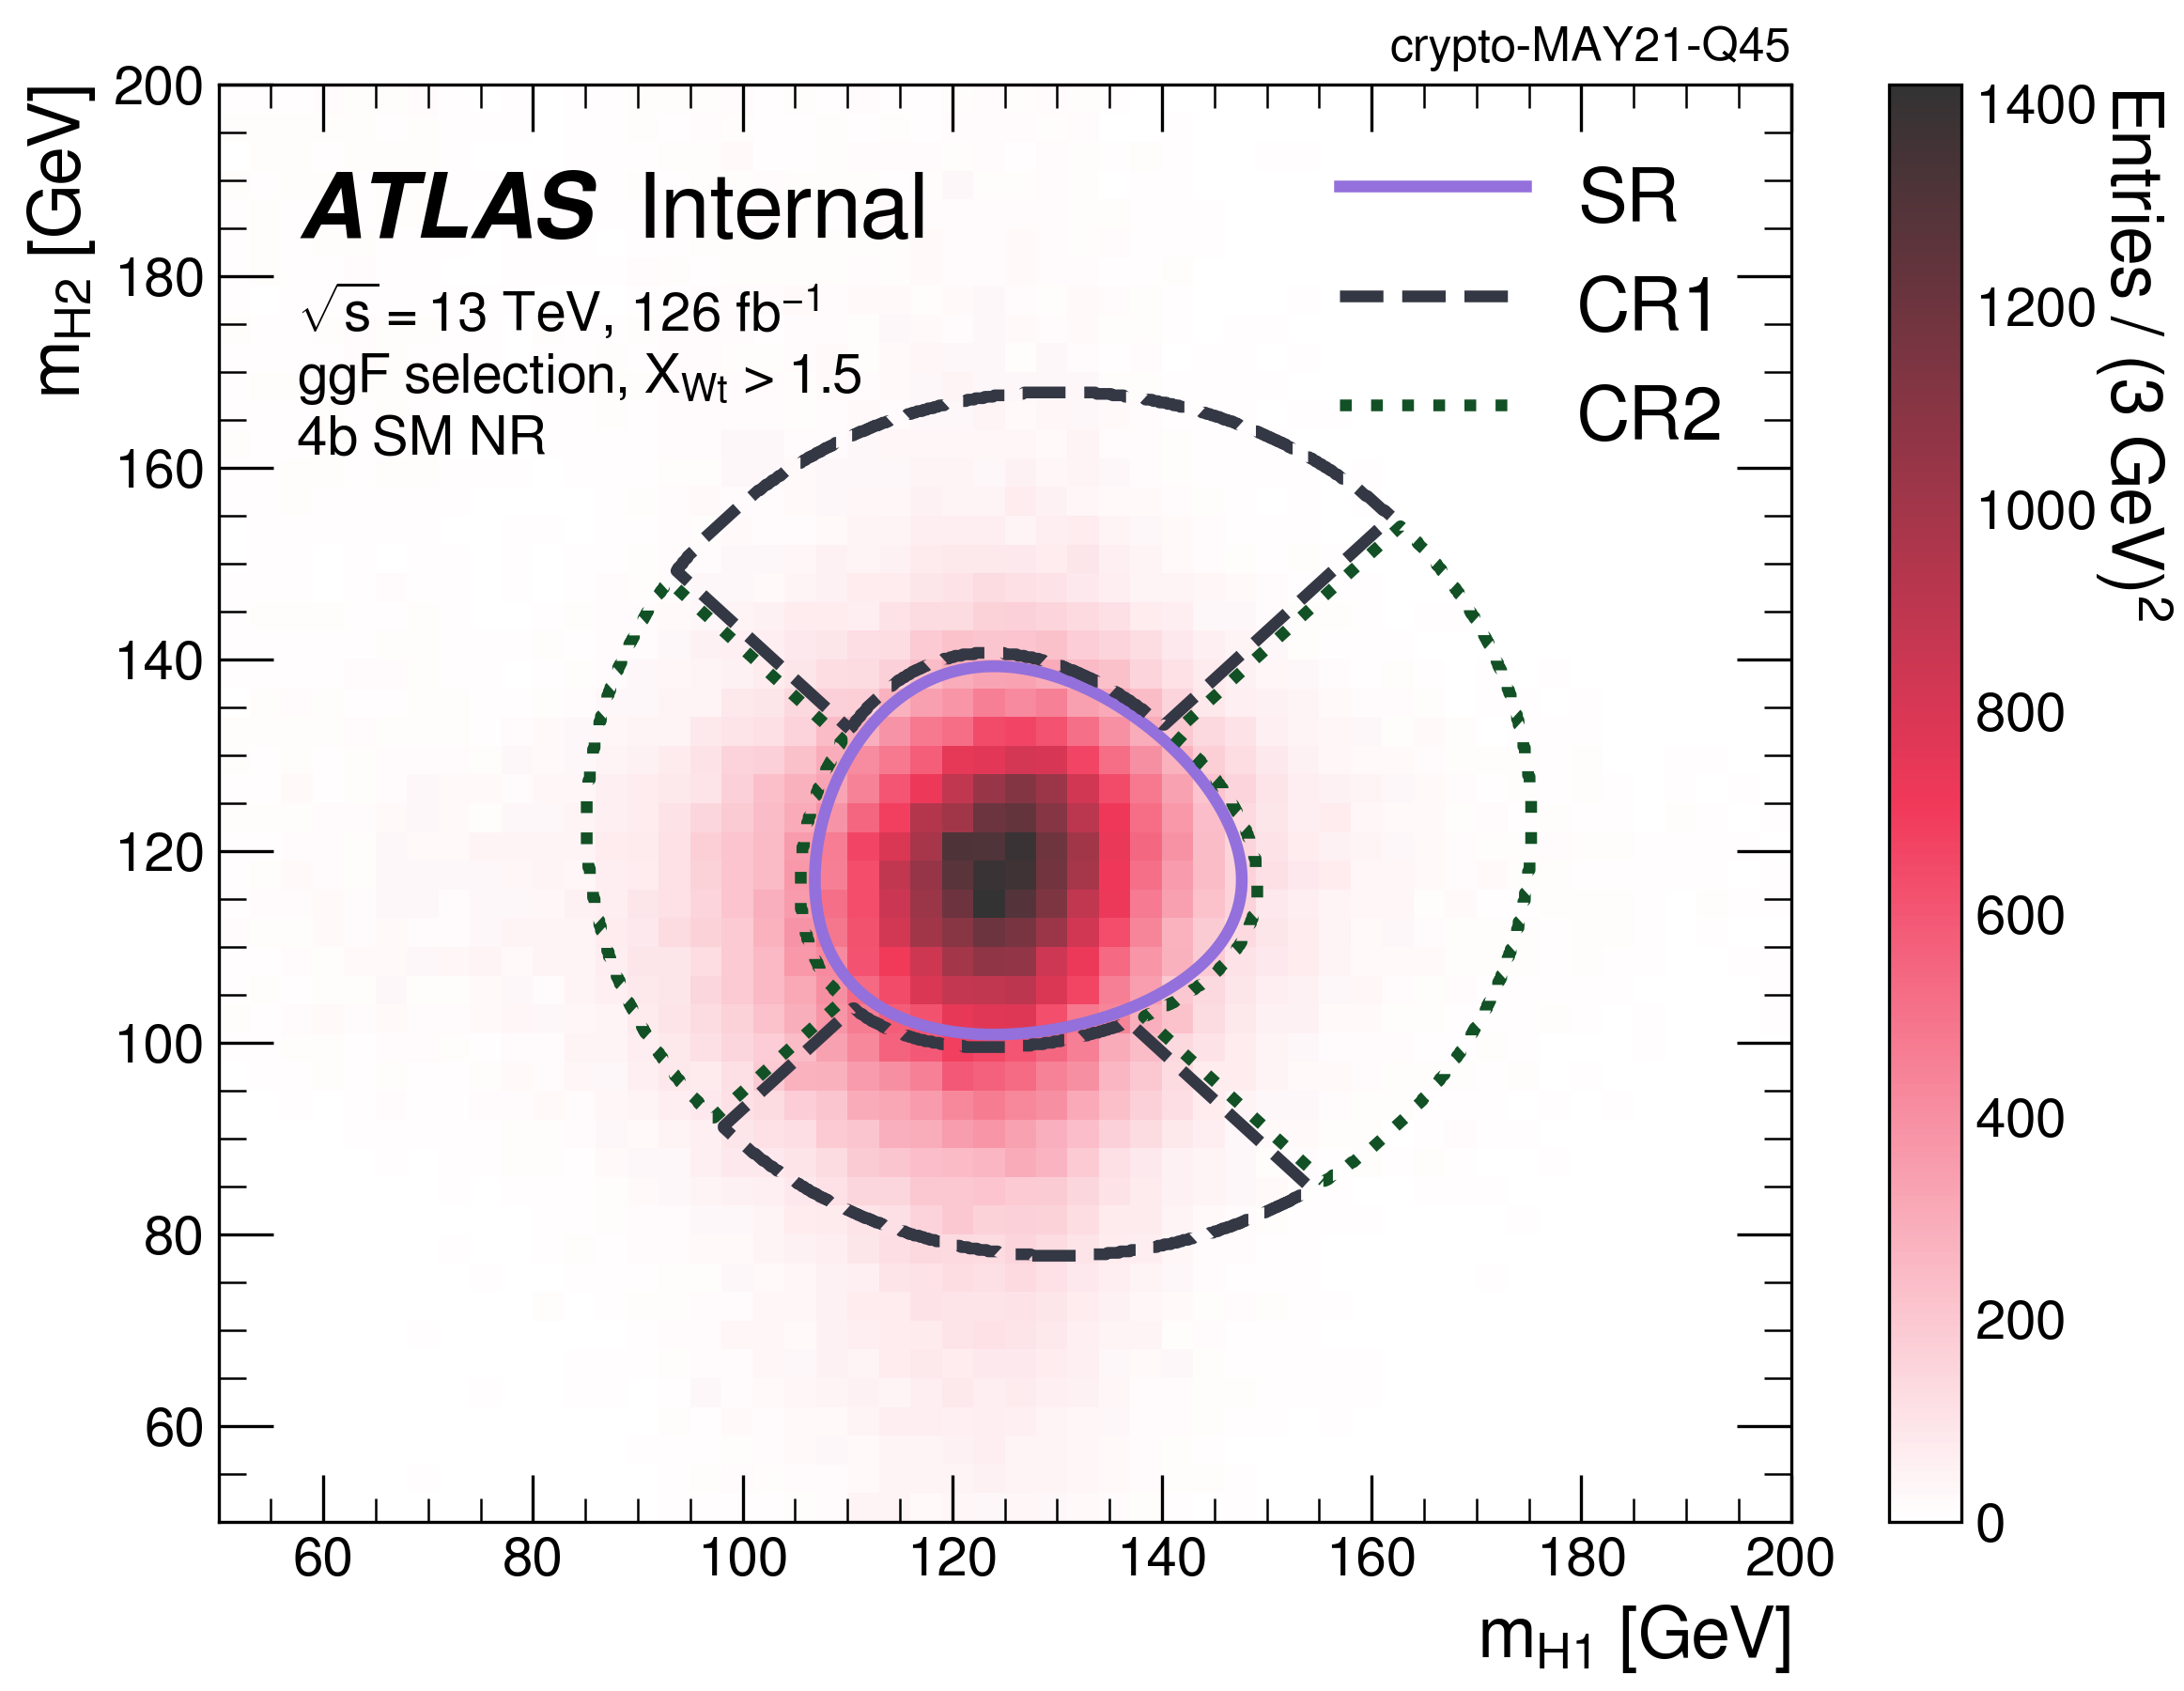
\includegraphics[width=0.4\textwidth]{figures/nr-int-note/selection/V3/massplane_sig_all_4b_ggf_Xwt_1.5.png}
		\label{fig:ggF-massplanes-allYrs-SM}
	}
	\subfloat[4b $\kappa_{2V} = 0$ signal]{ % with the VBF selection
	    	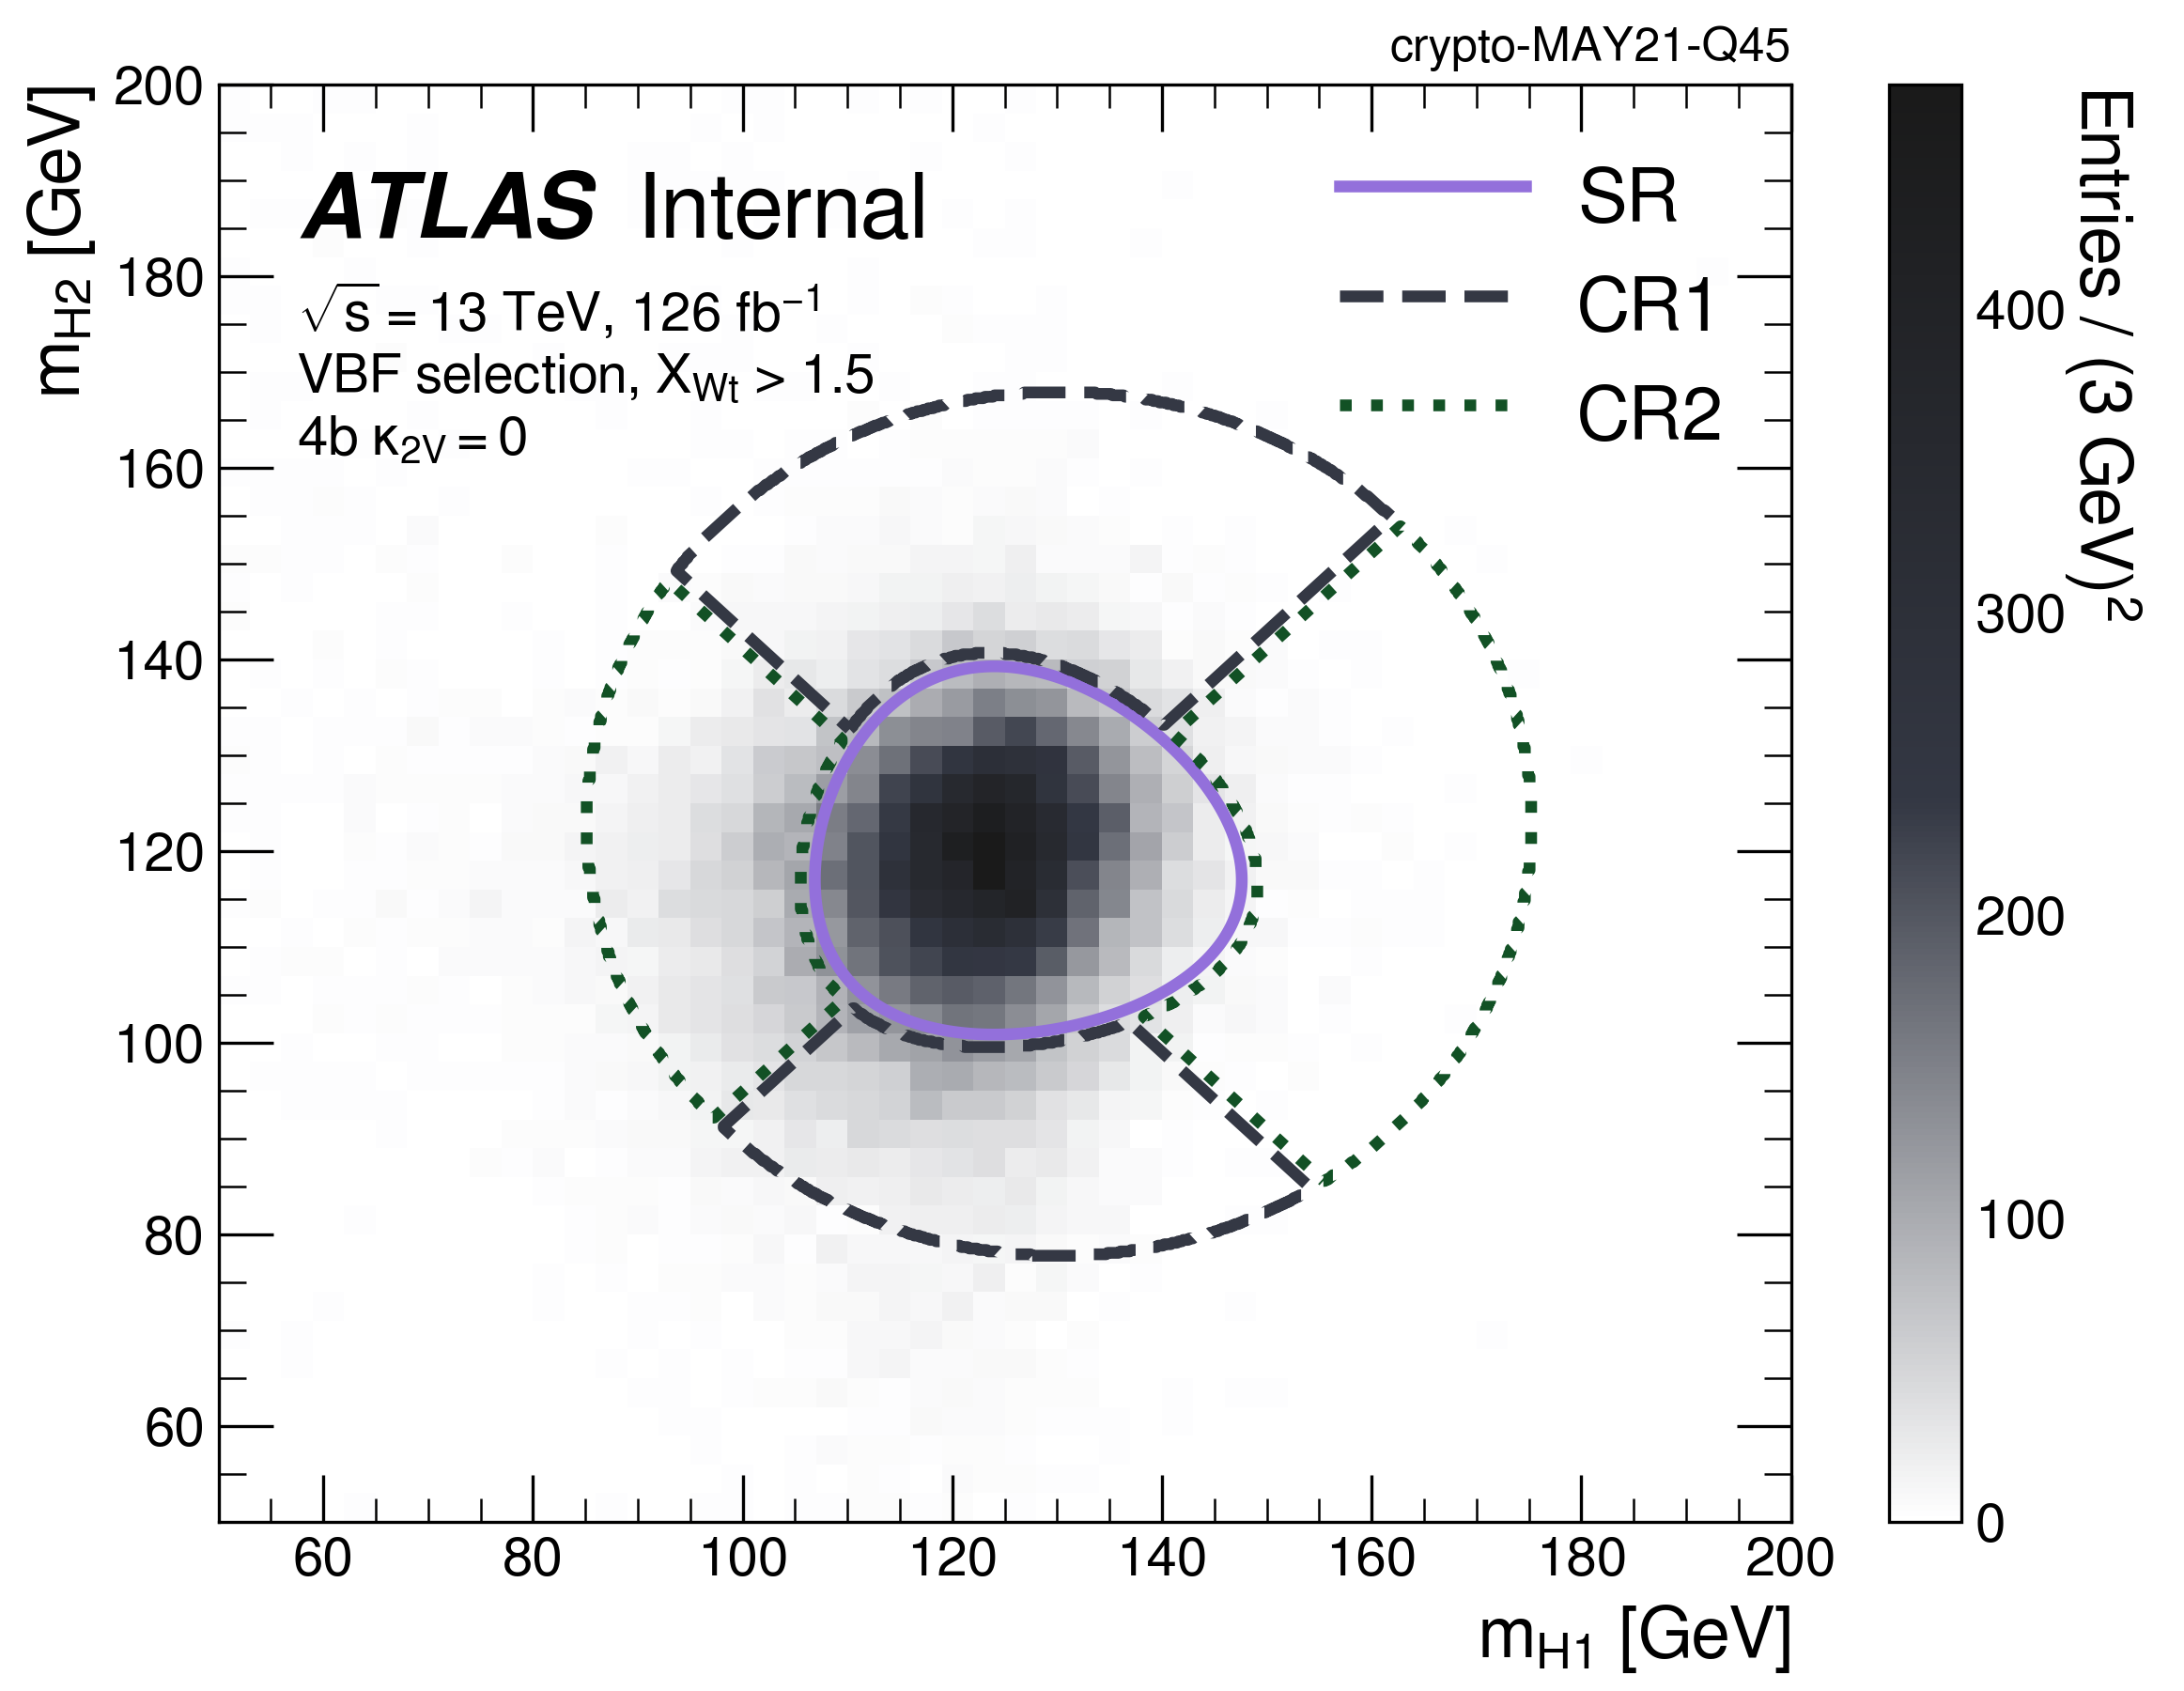
\includegraphics[width=0.4\textwidth]{figures/nr-int-note/selection/V3/massplane_sig_all_4b_vbf_Xwt_1.5_k2V_0.png}
 		\label{fig:VBF-massplanes-allYrs-k2V-0}
	}
	\caption{Selected Higgs Candidate signal mass planes.}
	\label{fig:massplanes-allYrs-signal}
\end{figure}

\begin{figure}[ht]
	\centering
	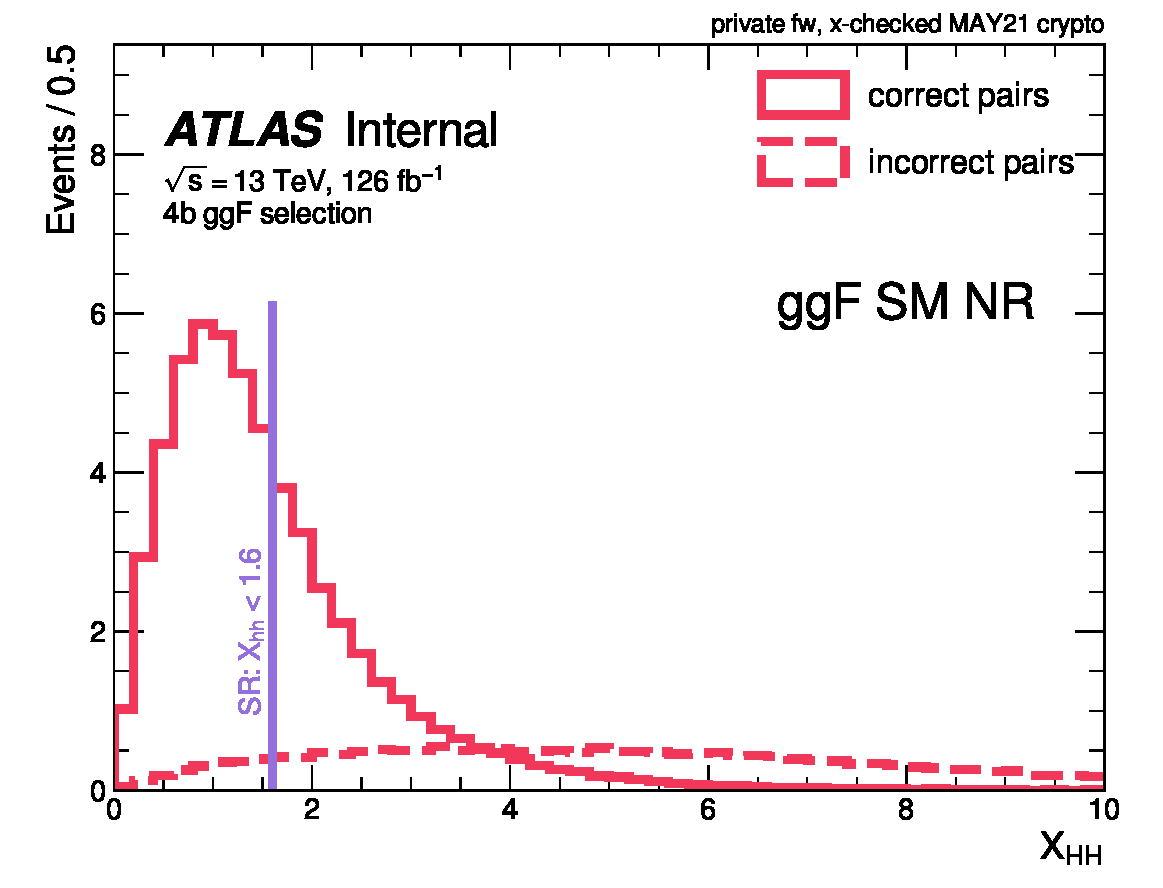
\includegraphics[width=0.4\textwidth]{figures/nr-int-note/selection/V3/X_hh-ggf-sm-4b.pdf}
	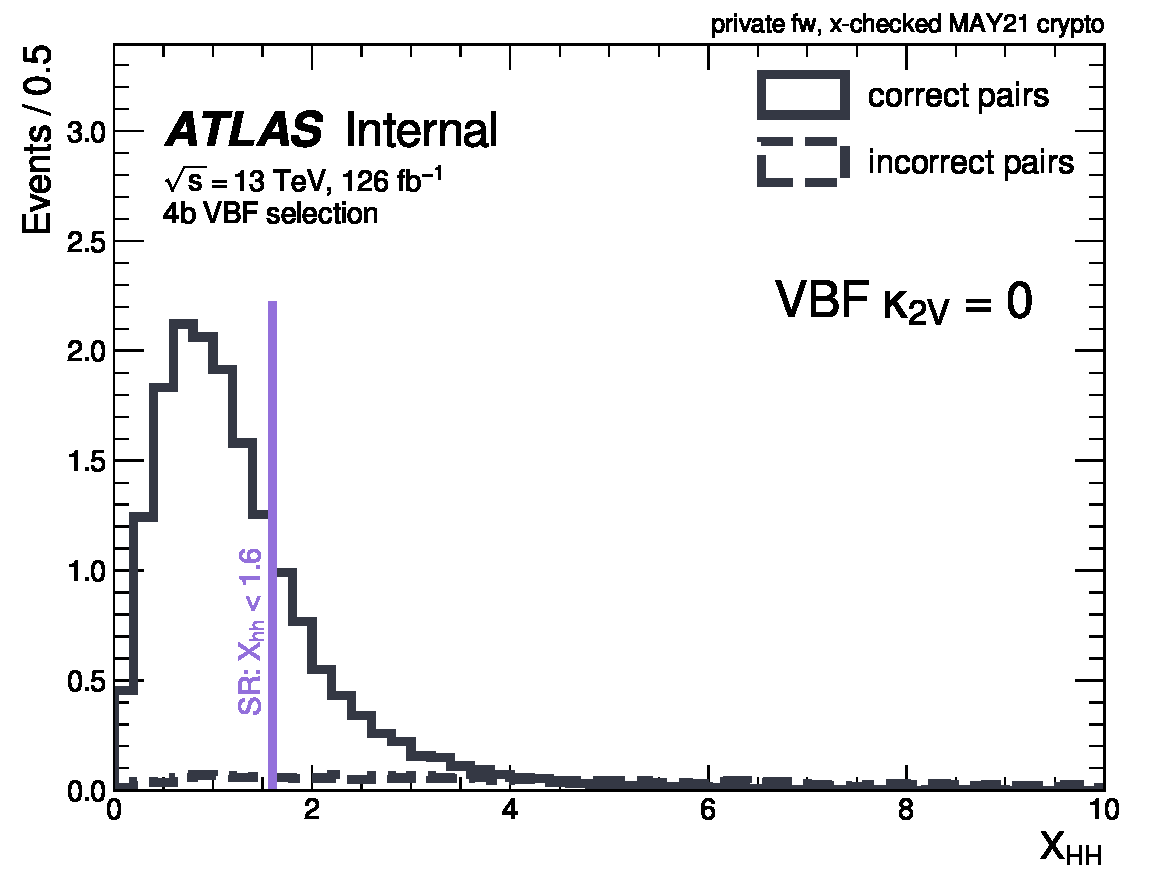
\includegraphics[width=0.4\textwidth]{figures/nr-int-note/selection/V3/X_hh-vbf-k2V_0-4b.pdf}
	\caption{Visualization of the \Xhh distribution for correctly and incorrectly paired events with the ggF (left) and VBF (right) analysis selections. The purple line indicates the SR defining cut.}
	\label{fig:ggF-Xhh}
\end{figure}

\begin{align}
	\text{SR} \quad &: \quad \Xhh < 1.6 \label{eq:sr} \\ 
	% \text{\textcolor{hh:darkblue}{CR1}/ \textcolor{hh:darkgreen}{CR2}}\ \text{Outer Edge} \quad &: \quad \sqrt{ \left(m_{\PH1} - 1.05 \cdot \SI{124}{\GeV}\right)^2 +  \left(m_{\PH2} - 1.05 \cdot \SI{117}{\GeV}\right)^2 } < \SI{45}{\GeV}  \label{eq:cr}
	\text{CR\ Inner\ Edge} \quad &: \quad \Xhh = 1.6 \label{eq:cr_in} \\
	\text{CR\ Outer\ Edge} \quad &: \quad \sqrt{ \left(m_{\PH1} - 1.05 \cdot \SI{124}{\GeV}\right)^2 +  \left(m_{\PH2} - 1.05 \cdot \SI{117}{\GeV}\right)^2 } = \SI{45}{\GeV}  \label{eq:cr_out}
\end{align}

\Fig{\ref{fig:massplanes-allYrs-data}} shows the blinded 4b data mass planes for the ggF and VBF selections, and the 2b data mass planes for the ggF and VBF selections. Note, the backgrounds for the 4b distributions are built from reweighted 2b data.

The key task for setting limits is correctly predicting the distributions for key discriminating variables in the SR. 
For this fully-hadronic final state analysis, we have a fully data driven background estimation method derived using events in a kinematically similar control region.
We define two control regions: Control Region 1 (CR1) and Control Region 2 (CR2). 
CR1 is used to derive the data-driven background estimate and CR2 is used to derive a systematic uncertainty associated with our methodology. 
These points will be expanded on in \Sect{\ref{sec:bkgdestimation}}. 
The region between the closed curves defined by \Eqn{\ref{eq:cr_in}} and \Eqn{\ref{eq:cr_out}} forms a band, within which CR1 and CR2 are defined. This region is orthogonal to the SR by design. This band is split into quadrants i.e. four sectors of roughly equal area. CR1 and CR2 are each defined as a pair of quadrants, where quadrants are paired such that they are on opposite sides of the band. The boundaries of CR1 and CR2 are shown in \Fig{\ref{fig:massplanes-allYrs-data}}.
This is a different choice comparing to the 4b resonant analysis~\cite{bbbbresolvedNote}, where rings of CR (and Validation Region) is used.
The new choice reduces potential signal contamination in resonant VR and has a better extrapolation since CR is closer to SR.
See \App{\ref{train-with-sig-inject}} for some studies.

\begin{figure}[ht]
	\centering
	\subfloat[Blinded 4b data for ggF selection]{
	     	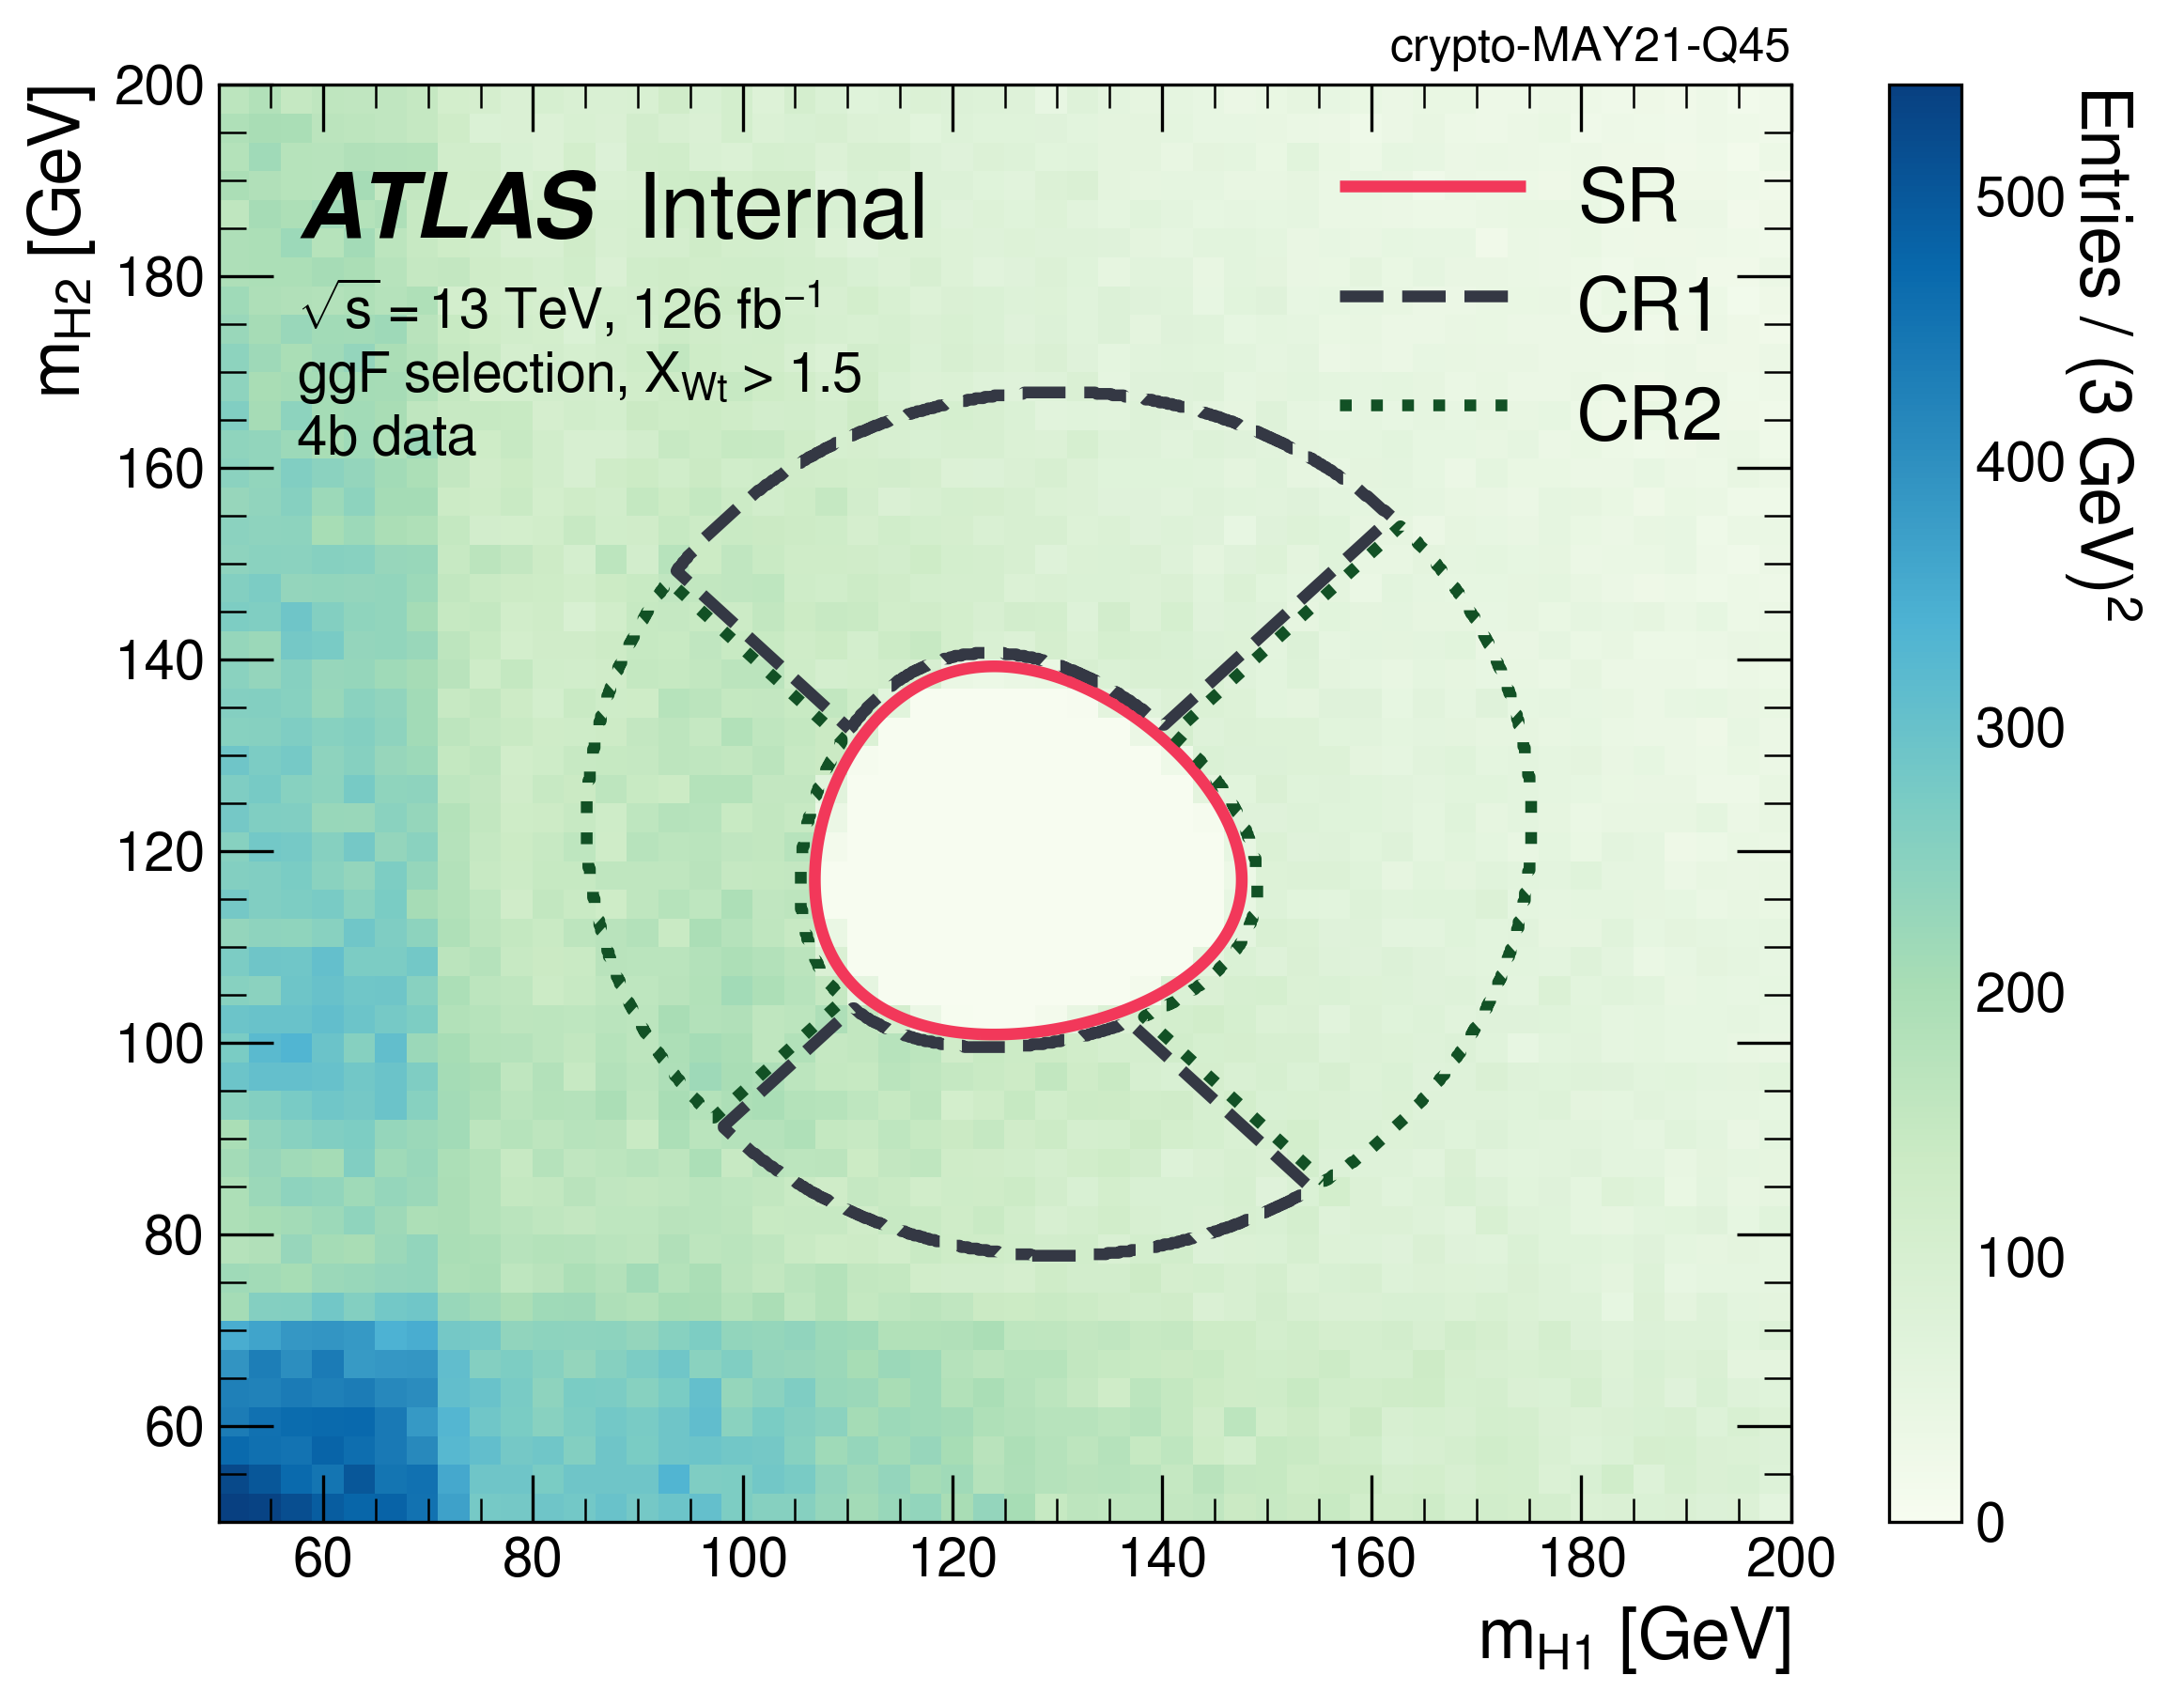
\includegraphics[width=0.4\textwidth]{figures/nr-int-note/selection/V2/massplane_dat_all_4b_ggf_Xwt_1.5.png}
		\label{fig:ggF-massplanes-allYrs-dat-4b}
	}
	\subfloat[Blinded 4b data for VBF selection]{
	     	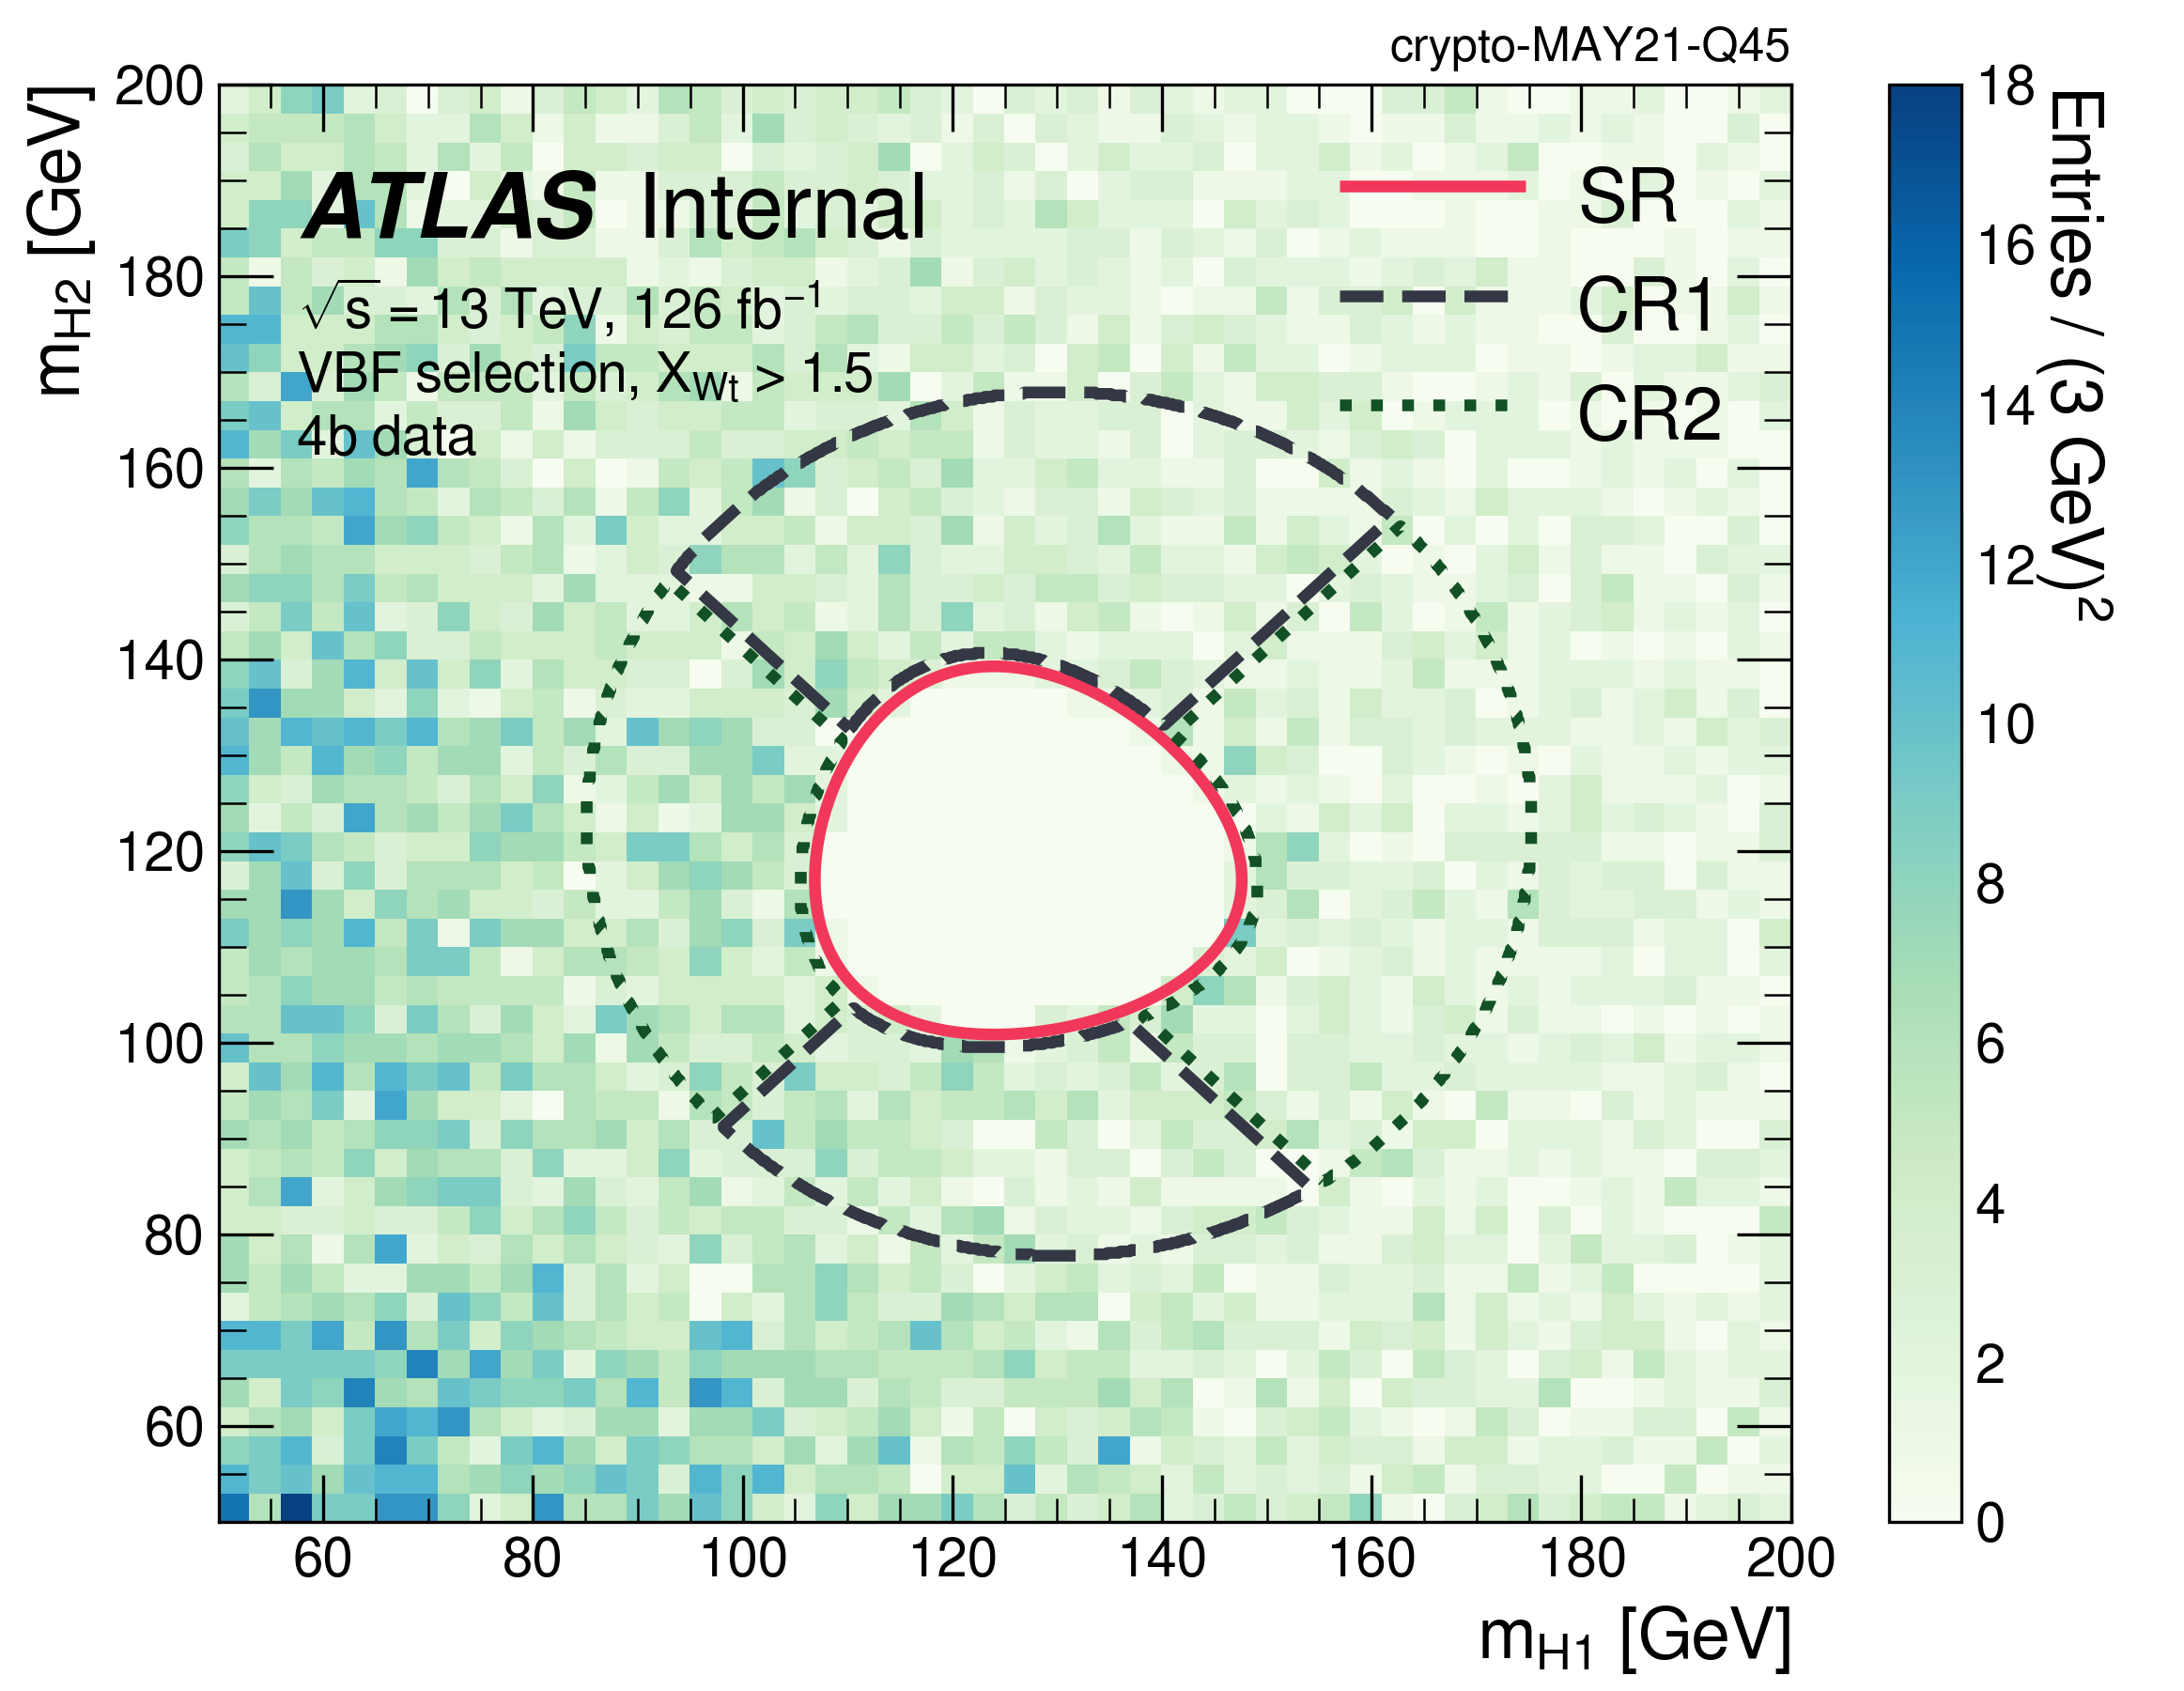
\includegraphics[width=0.4\textwidth]{figures/nr-int-note/selection/V2/massplane_dat_all_4b_vbf_Xwt_1.5.png} 
		\label{fig:VBF-massplanes-allYrs-dat-4b}
	}\\
	\centering
	\subfloat[2b data for ggF selection]{
	     	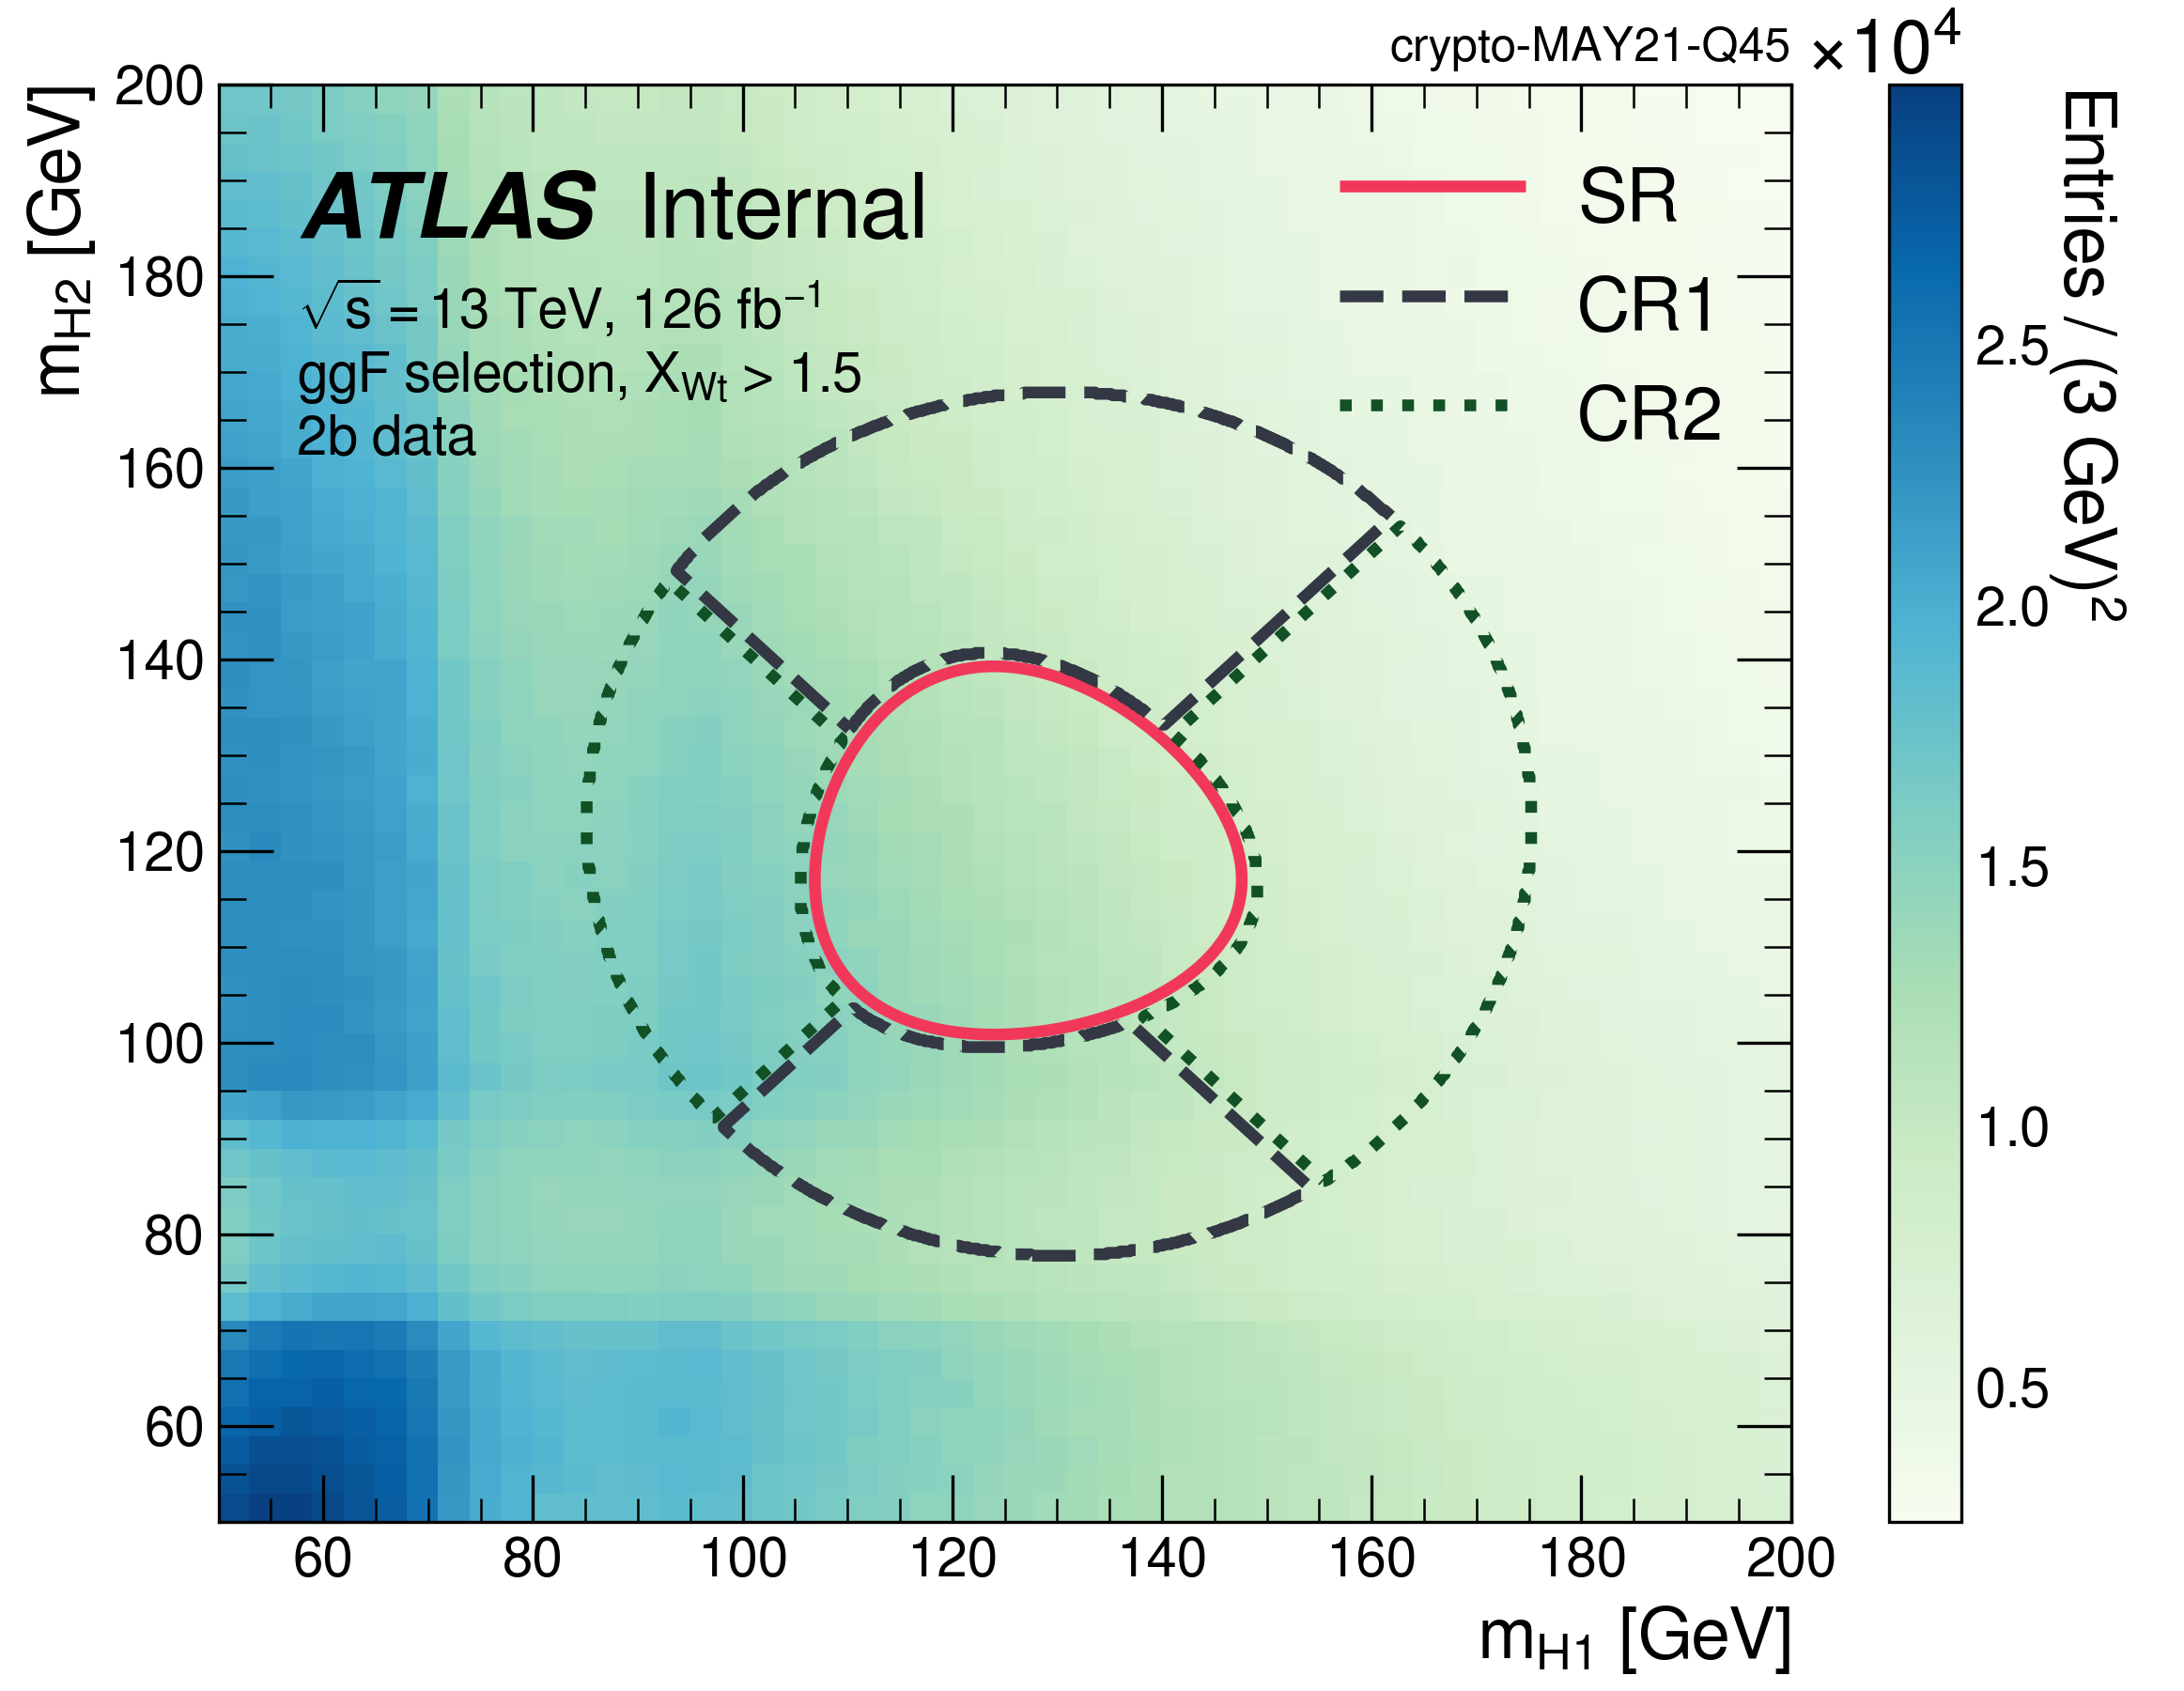
\includegraphics[width=0.4\textwidth]{figures/nr-int-note/selection/V2/massplane_dat_all_2b_ggf_Xwt_1.5.png}
		\label{fig:ggF-massplanes-allYrs-dat-2b}
	}
	\subfloat[2b data for VBF selection]{
	     	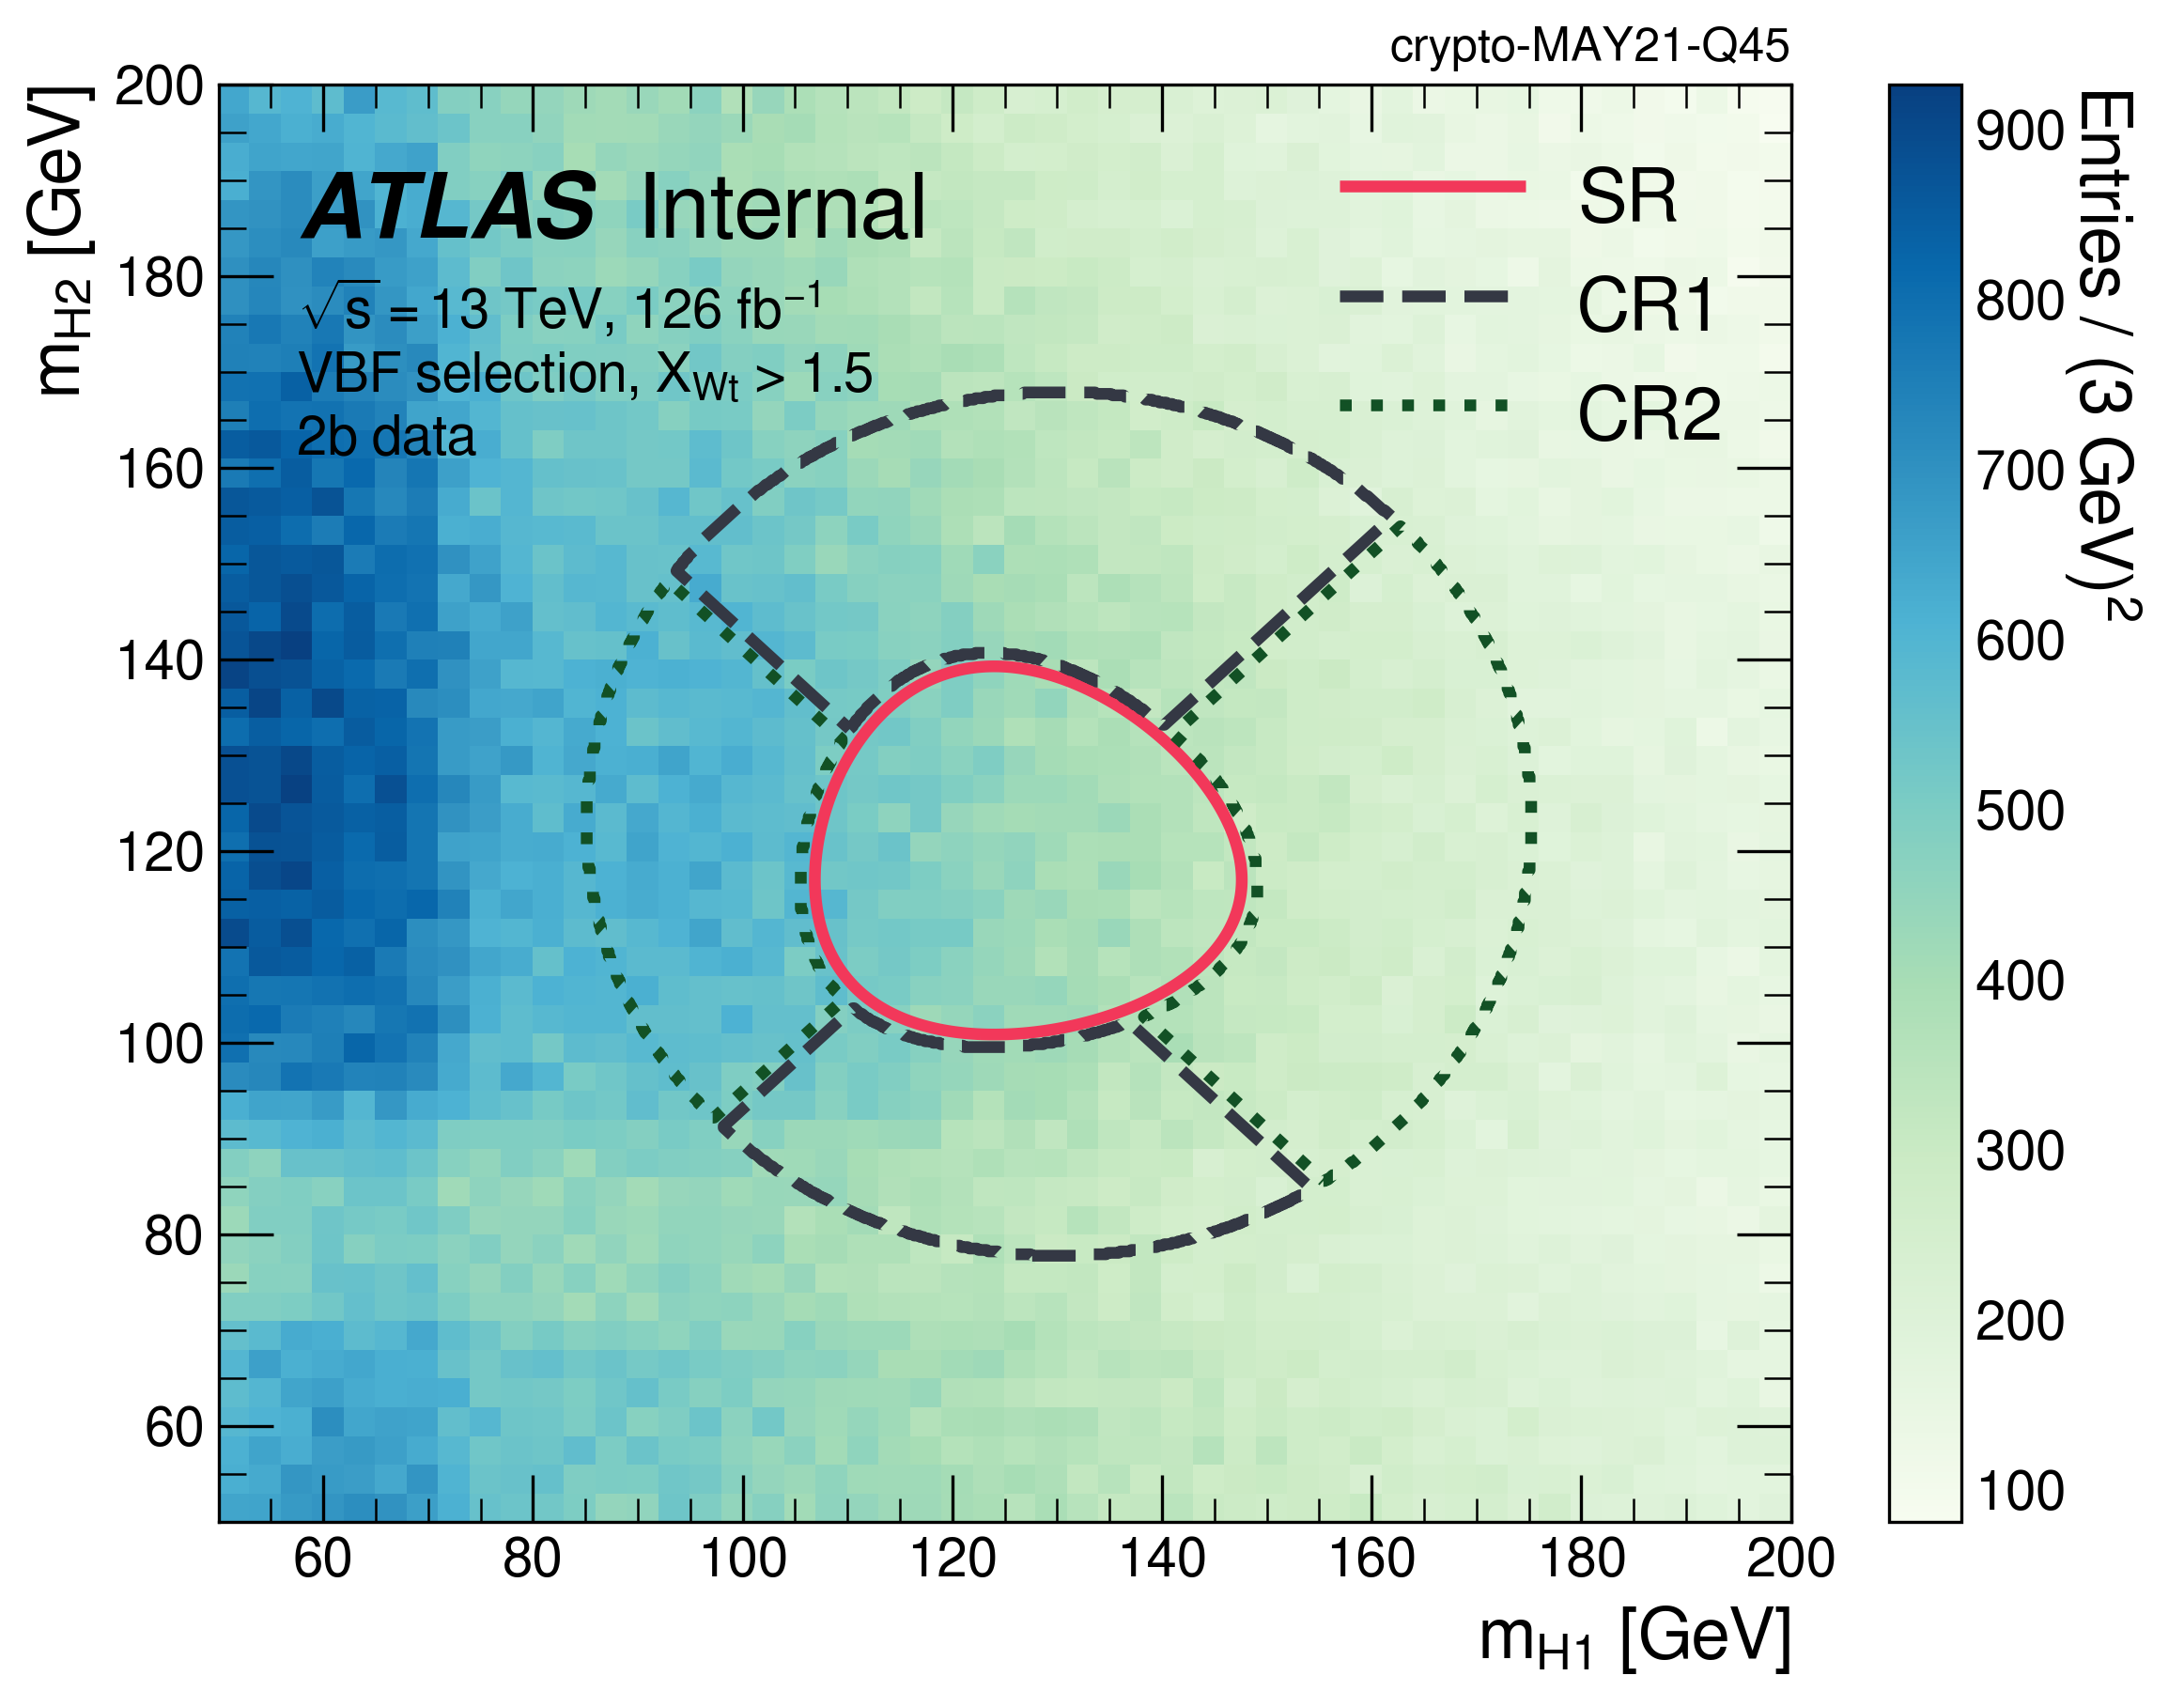
\includegraphics[width=0.4\textwidth]{figures/nr-int-note/selection/V2/massplane_dat_all_2b_vbf_Xwt_1.5.png} 
		\label{fig:VBF-massplanes-allYrs-dat-2b}
	}
	\caption{The Higgs Candidate massplanes for the ggF and VBF analysis selections.}
	\label{fig:massplanes-allYrs-data}
\end{figure}

The four quadrants that define CR1 and CR2 can be orientated in an infinite number of ways. The \Xwt cut applied in the selection acts like a \PW-mass veto for the constructed Higgs Candidates (HCs) causing a distinct drop in the number of events with $m_{h1}$ or $m_{h2}$ equal to $\sim$80 \GeV. In \Fig{\ref{fig:massplanes-allYrs-data}}, this effect can be observed as the two straight light-colored bands centered around $\sim$80 \GeV on the x and y-axes which stretch horizontally and vertically across the plot.\footnote{These mass planes before applying the \Xwt > 1.5 cut are shown in \Fig{\ref{fig:ggF-massplanes-Xwt}} and \Fig{\ref{fig:VBF-massplanes-Xwt}} for the respective ggF and VBF selections} The orientation of the quadrants shown in \Fig{\ref{fig:massplanes-allYrs-data}} was chosen such that these dips in the number of events equally impacted both CR1 and CR2.

Several different orientations were tested. In the studies conducted, different orientations were expressed as the angle between the x-axis and the closest CR1-CR2 boundary above the x-axis. Angles of \SI{0}{\degree}, \SI{30}{\degree}, \SI{45}{\degree} were compared and \SI{45}{\degree} was found to give better agreement 
in the 3b + 1 fail validation sample. Further investigation showed that this improvement stems from the \Xwt variable similarity, which is discussed in \App{\ref{app:sec:emd}}.

%CRs are defined by events passing the selection in \Eqn{\ref{eq:cr}}, where the steeply falling mass planes in \Fig{\ref{fig:massplanes-allYrs-data}} motivate the additional shift of 1.05 for the circle center for the means of the $(m_{H1}, m_{H2})$ 2b distributions to approximately match the 2b SR means. \todo{Need to check if this statement is still true with the new regions, or remove this motivation for the 1.05 shift.}
